% This is a Basic Assignment Paper but with code, URLs, and hyperlinks included.

\documentclass[openany]{report}

% Preamble

\usepackage[margin=1in]{geometry}
\usepackage{amsfonts, amsmath, amssymb}
\usepackage{fancyhdr, float, graphicx}
\usepackage[utf8]{inputenc} % For international characters
\usepackage[T1]{fontenc}    % Output font encoding
\usepackage{fouriernc}      % New Century Schoolbook font
\usepackage[nottoc, notlot, notlof]{tocbibind}
\usepackage{listings}
\usepackage{xcolor}
\usepackage{hyperref}

\hypersetup{
    colorlinks=true,
    linkcolor=black,
    filecolor=magenta,
    urlcolor=blue,
    pdfpagemode=FullScreen,
}

\definecolor{codegreen}{rgb}{0,0.6,0}
\definecolor{codegray}{rgb}{0.5,0.5,0.5}
\definecolor{codepurple}{rgb}{0.58,0,0.82}
\definecolor{backcolour}{rgb}{0.95,0.95,0.92}

\lstdefinestyle{mystyle}{
    backgroundcolor=\color{backcolour},
    commentstyle=\color{codegreen},
    keywordstyle=\color{magenta},
    numberstyle=\tiny\color{codegray},
    stringstyle=\color{codepurple},
    basicstyle=\ttfamily\footnotesize,
    breaklines=true,
    captionpos=b,
    numbers=left,
    numbersep=5pt,
    tabsize=2,
    showspaces=false,
    showstringspaces=false,
    showtabs=false
}

\lstset{style=mystyle}

% Header and Footer
\pagestyle{fancy}
\fancyhead{}
\fancyfoot{}
\fancyhead[L]{\textit{\Large{Report - 4th Year B. Tech}}}
\fancyhead[R]{\textit{Krishnaraj Thadesar}}
\fancyfoot[C]{\thepage}
\renewcommand{\footrulewidth}{1pt}

\begin{document}

%----------------------------------------
\chapter{Individual Contribution}
%----------------------------------------
\section{Problem Statement}
Design and implement the backend API and face‐recognition engine for the Attendance‐Assistant system.

\section{Student Details}
\textbf{Krishnaraj Thadesar} \\
\textbf{PRN:} 1032210888 \\
\textbf{Roll Number:} 15 \\
\textbf{Panel:} A \\

\section{Module Title}
Backend \& Face-Recognition Engine

\begin{figure}[H]
    \centering
    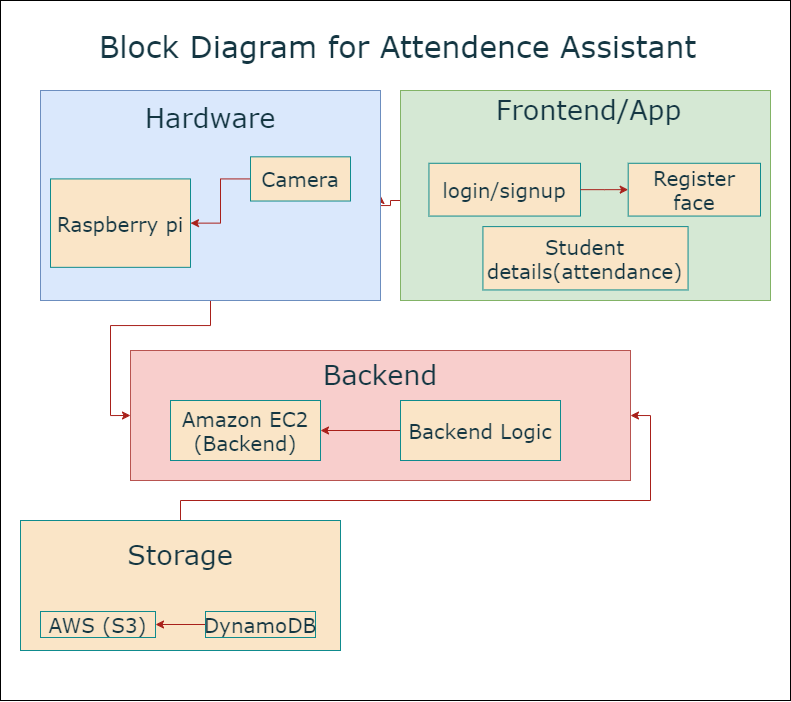
\includegraphics[width=0.95\textwidth]{../imgs/block diagram.png}
    \caption{Block Diagram highlighting the backend \& face‐recognition module (Krishnaraj Thadesar’s contribution).}
    \label{fig:block_diagram_krishnaraj}
\end{figure}

\section{Project Module Scope}
End-to-end implementation of backend services, face-encoding storage and lookup, and concurrent API handling.

\section{Project Modules – Individual Contribution}
\begin{enumerate}
  \item \textbf{Hardware \& Software requirements:} PC (i7,16 GB RAM), server (4 vCPU,8 GB RAM); Python 3.9, FastAPI, face\_recognition, Docker, MongoDB.
  \item \textbf{Module Interfaces:} 
    \begin{itemize}
      \item POST \texttt{/api/auth/login}
      \item POST \texttt{/api/faces/encode}
      \item POST \texttt{/api/attendance/mark}
      \item GET  \texttt{/api/reports/daily}
    \end{itemize}
  \item \textbf{Module Dependencies:} face\_recognition→dlib, numpy; FastAPI→uvicorn, pydantic; motor (MongoDB driver).
  \item \textbf{Module Design:} Controller→Service→Model→Persistence layers; singleton model loader; JWT auth.
  \item \textbf{Module Implementation:} Docker Compose, ~1,200 LOC Python, integrated ResNet-based pipeline.
  \item \textbf{Testing Strategies:} pytest (>=85\% coverage), mocked CI tests, Postman smoke tests.
  \item \textbf{Deployment:} Docker Compose (dev), AWS ECR/ECS Fargate (prod), auto-scaling.
\end{enumerate}

\chapter{Individual Contribution}

\section{Problem Statement}
Provision and orchestrate basic cloud infrastructure, CI/CD pipelines, and support backend rollout.

\section{Student Details}
\textbf{Parth Zarekar} \\
\textbf{PRN:} 1032210846 \\
\textbf{Roll Number:} 09 \\
\textbf{Panel:} A \\

\section{Module Title}
Cloud Infrastructure \& CI/CD Support

\begin{figure}[H]
  \centering
  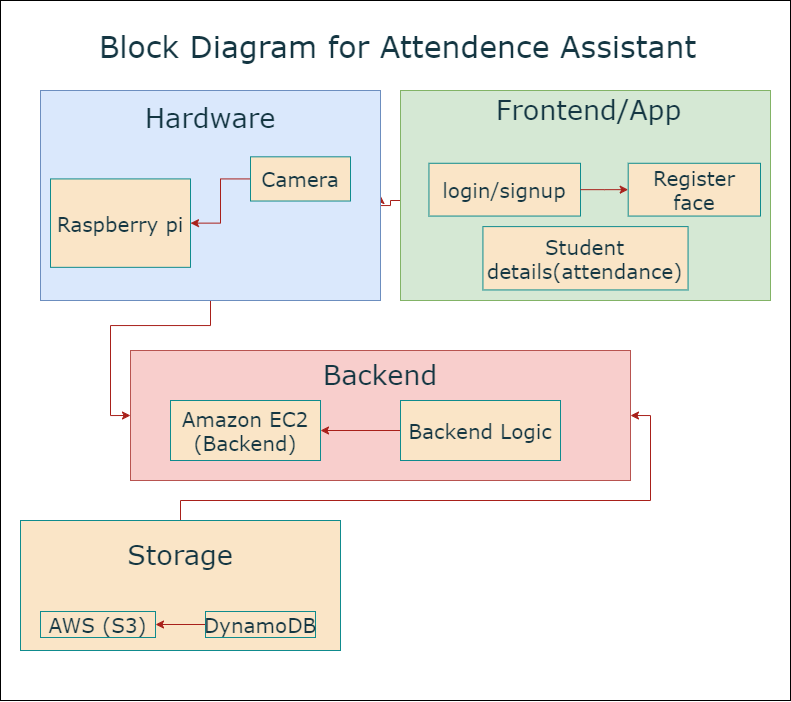
\includegraphics[width=0.95\textwidth]{../imgs/block diagram.png}
  \caption{Block Diagram highlighting the infrastructure \& CI/CD portion (Parth Zarekar’s contribution).}
  \label{fig:block_diagram_parth}
\end{figure}

\section{Project Module Scope}
Basic AWS setup and DynamoDB usage; CI/CD pipeline configuration; backend image-upload research; documentation support.

\section{Project Modules – Individual Contribution}
\begin{enumerate}
  \item \textbf{Cloud \& Storage:} Stand up a simple AWS EC2 instance and DynamoDB table for attendance data.
  \item \textbf{CI/CD Pipeline:} Configure GitHub Actions to build, test, and deploy backend Docker images.
  \item \textbf{Research \& Documentation:}
    \begin{itemize}
      \item Explored MongoDB integrations for image storage.
      \item Assisted in drafting sections of the research paper and user documentation.
      \item Provided Figma feedback for UI wireframes.
    \end{itemize}
\end{enumerate}

%----------------------------------------
\chapter{Individual Contribution}
%----------------------------------------
\section{Problem Statement}
Evaluate and benchmark multiple face-recognition algorithms; support model selection and integration.

\section{Student Details}
\textbf{Sourab Karad} \\
\textbf{PRN:} 1032211150 \\
\textbf{Roll Number:} 40 \\
\textbf{Panel:} A \\

\section{Module Title}
Algorithm Research \& Model Integration

\begin{figure}[H]
    \centering
    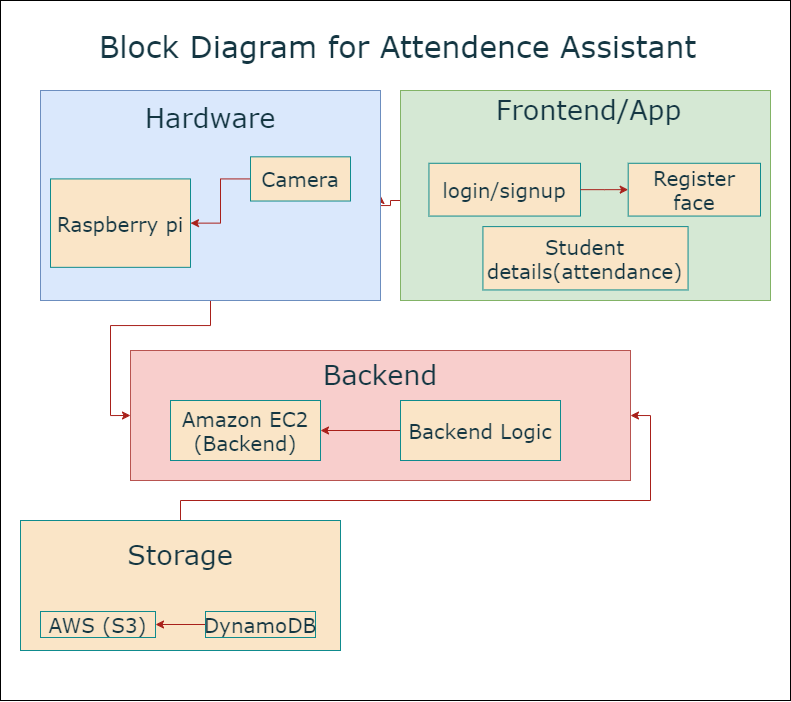
\includegraphics[width=0.95\textwidth]{../imgs/block diagram.png}
    \caption{Block Diagram highlighting the algorithm research module (Sourab Karad’s contribution).}
    \label{fig:block_diagram_sourab}
\end{figure}

\section{Project Module Scope}
Implementation and evaluation of face-recognition methods; performance reporting and API stub delivery.

\section{Project Modules – Individual Contribution}
\begin{enumerate}
  \item \textbf{Hardware \& Software requirements:} GPU (RTX 2060), dlib, OpenCV, torch, scikit-learn, pandas.
  \item \textbf{Module Interfaces:} \texttt{train\_model.py}, \texttt{evaluate.py}; JSON output (\texttt{accuracy, precision, recall}).
  \item \textbf{Module Dependencies:} torch→torchvision; face\_recognition→dlib; numpy→pandas.
  \item \textbf{Module Design:} Abstract base classes; modular trainer \& evaluator.
  \item \textbf{Module Implementation:} ~800 LOC benchmarking harness; comparative plots in report.
  \item \textbf{Testing Strategies:} 5-fold cross-validation; confusion matrices.
  \item \textbf{Deployment:} Packaged ResNet model as pickle; provided Dockerfile snippet.
\end{enumerate}

%----------------------------------------
\chapter{Individual Contribution}
%----------------------------------------
\section{Problem Statement}
Design and build the cross-platform mobile app for attendance marking via facial capture.

\section{Student Details}
\textbf{Saubhagya Singh} \\
\textbf{PRN:} 1032211144 \\
\textbf{Roll Number:} 38 \\
\textbf{Panel:} A \\

\section{Module Title}
Flutter Front-End Application

\begin{figure}[H]
    \centering
    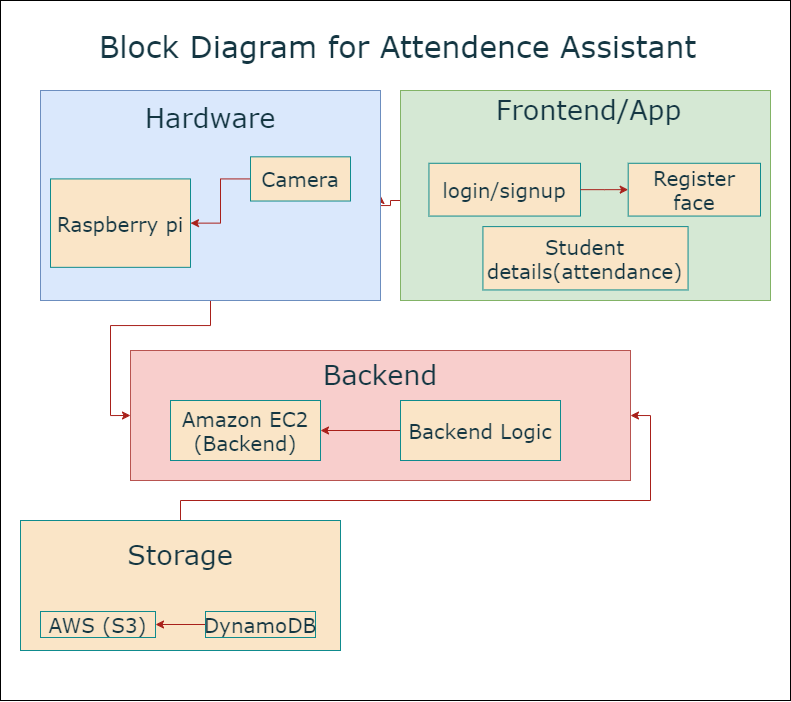
\includegraphics[width=0.95\textwidth]{../imgs/block diagram.png}
    \caption{Block Diagram highlighting the frontend module (Saubhagya Singh’s contribution).}
    \label{fig:block_diagram_saubhagya}
\end{figure}

\section{Project Module Scope}
Full-featured Flutter app: login, camera capture, attendance history, offline caching.

\section{Project Modules – Individual Contribution}
\begin{enumerate}
  \item \textbf{Hardware \& Software requirements:} Android/iOS device or emulator; Flutter 3.x, Dart, Android Studio, Xcode.
  \item \textbf{Module Interfaces:} Flutter HTTP client→\texttt{POST /api/faces/encode}; Provider state management.
  \item \textbf{Module Dependencies:} \texttt{camera}, \texttt{image\_cropper}, \texttt{flutter\_secure\_storage}, \texttt{sqflite}.
  \item \textbf{Module Design:} MVVM pattern; widget tree: Login→CameraView→AttendanceList.
  \item \textbf{Module Implementation:} ~1\,500 LOC Dart; custom camera overlay; retry logic.
  \item \textbf{Testing Strategies:} Widget tests; Flutter Driver integration tests.
  \item \textbf{Deployment:} GH Actions→TestFlight \& Play Store via Fastlane.
\end{enumerate}

\end{document}
